%===============================================================================
% Poster
%===============================================================================
% $Id: poster.tex 248 2005-01-30 23:25:27Z thom $
%===============================================================================


%===============================================================================
% Configuration
%===============================================================================


%-------------------------------------------------------------------------------
% \documentclass and \usepackage directives
%-------------------------------------------------------------------------------
\documentclass[a0,portrait]{a0poster}
\usepackage{times,colordvi,amsmath,epsfig,float,color,multicol}
\usepackage[latin1]{inputenc}
\usepackage[T1]{fontenc}


%-------------------------------------------------------------------------------
% Colors
%-------------------------------------------------------------------------------
% PMS287 CMYK=[100% 69% 0% 11.5%] RGB=[38/256 67/256 151/256]
\definecolor{qmuldarkblue}{rgb}{0.1484375,0.26171875,0.58984375}

\definecolor{backgrey}{rgb}{0.93,0.93,0.93}
\definecolor{backblue}{rgb}{0.93,0.93,1}
\definecolor{backyellow}{rgb}{1,1,0.88} 

\definecolor{backred}{rgb}{1,0.9,0.9} 
\definecolor{backgreen}{rgb}{0.9,1,0.9}
\definecolor{backpink}{rgb}{1,0.9,1} 
\definecolor{backturquoise}{rgb}{0.9,1,1}


%-------------------------------------------------------------------------------
% Common configuration
%-------------------------------------------------------------------------------
\pagestyle{empty}
\setlength{\parindent}{0cm}
\setlength{\parskip}{2ex}
\setlength{\columnsep}{3cm}
\addtolength{\textwidth}{2cm}
\addtolength{\oddsidemargin}{-1.5cm}


%-------------------------------------------------------------------------------
% Commandos
%-------------------------------------------------------------------------------
\renewcommand{\normalsize}{\Large}
\def\regularsize{\@setfontsize\normalsize{34pt}{37}}

\renewcommand\refname{}
\setlength{\fboxrule}{0.1cm}

\makeatletter
\renewcommand{\section}{\@startsection
  {section}                          % the name 
  {1}                                % the level
  {0mm}                              % the indent
  {-0.7\baselineskip}                % the beforeskip
  {5mm}                              % the afterskip
  {\center\Huge\color{qmuldarkblue}\bfseries}} % the style
\makeatother


%===============================================================================
% Document
%===============================================================================
\begin{document}

\vspace{1cm}


%-------------------------------------------------------------------------------
% Header
%-------------------------------------------------------------------------------
\begin{center}
\colorbox{qmuldarkblue} { 

  \color{white}
    
  \parbox{1.0\textwidth} 
  { 
    \parbox{0.24\textwidth} 
    {
      \begin{center}
        
      \end{center}
    } 
    \parbox{0.5\textwidth} 
    { 
      \vspace{1cm}
      \begin{center}
        \textrm 
        {
          {\veryHuge \bf \em EiffelRSS}\\[1ex]
          {\huge Michael K�ser, Martin Luder, Thomas Weibel} 
        }
      \end{center}
      \vspace{1cm} 
    } 
    \parbox{0.24\textwidth} 
    {
      \begin{center}
        
      \end{center}
    } 
  } 
}
\end{center}


\vspace{1cm}


%-------------------------------------------------------------------------------
% Sections
%-------------------------------------------------------------------------------
\begin{multicols}{2}

  \fcolorbox{black}{backblue}
  {
    \parbox{1.0\columnwidth}
    {
      \section*{What is EiffelRSS?}

      \begin{itemize}
      \item EiffelRSS is an Eiffel library to read and write RSS. The
        goal is to provide the Eiffel development community with an
        easy to use and well structured API for RSS.
      \item The distribution also contains a RSS newsfeed reader
        written with \\ EiffelVision and EiffelRSS.
      \end{itemize}
    }
  }
  
  \vspace{1cm}

  \fcolorbox{black}{backblue}{
    \parbox{1.0\columnwidth}
    {
      \section*{EiffelRSS Library}

      Clusters:

      \begin{itemize}
      \item \texttt{ADT} features classes to implement sortable
        structures.
      \item \texttt{FETCH} can fetch data from a source address to a
        local \texttt{STRING} using HTTP, FTP and file.
      \item \texttt{LOGFILE} represents a file which can be used for
        logging messages during the program execution.
      \item \texttt{PROPERTIES} represents a persistent set of
        properties.
      \item \texttt{SYNDICATION} is the main cluster of EiffelRSS with
        a feed object model, and classes to load and write feeds. It
        has three subcusters:
        \begin{itemize}
        \item \texttt{INTERFACE} contains all the classes a developer
          needs to use the library.
        \item \texttt{FEED} is the central datastructure of EiffelRSS.
          It defines an abstract syndication feed.
        \item \texttt{FORMATS} defines the different syndication
          formats. It is easy extensible with other formats.
        \end{itemize}
      \end{itemize}
      
      \begin{center}
        \resizebox*{\columnwidth}{!}{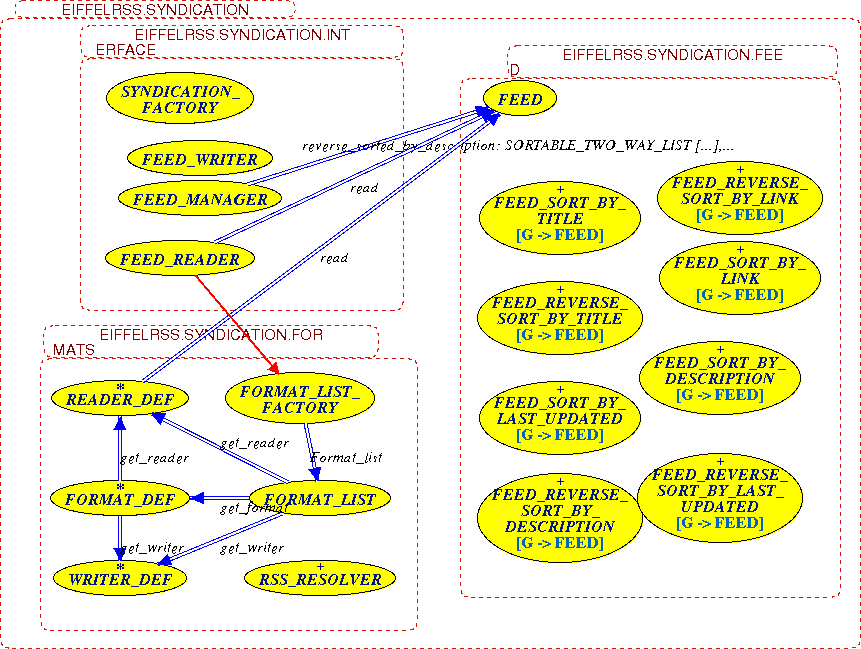
\includegraphics{figures/EIFFELRSS_SYNDICATION}}
      \end{center}
    }
  }
  
  \vspace{1cm}

  \fcolorbox{black}{backblue}{
    \parbox{1.0\columnwidth}
    {
      \section*{EiffelRSS Newsreader}

      \begin{itemize}
      \item Newsreader is a simple RSS-feed reader which shows the
        possibilities of the EiffelRSS library.
      \item You can add custom feeds and open news in your Internet
        browser.
      \item Features a graphical and command line user interface.
      \end{itemize}

      \begin{center}
        \resizebox*{0.85\columnwidth}{!}{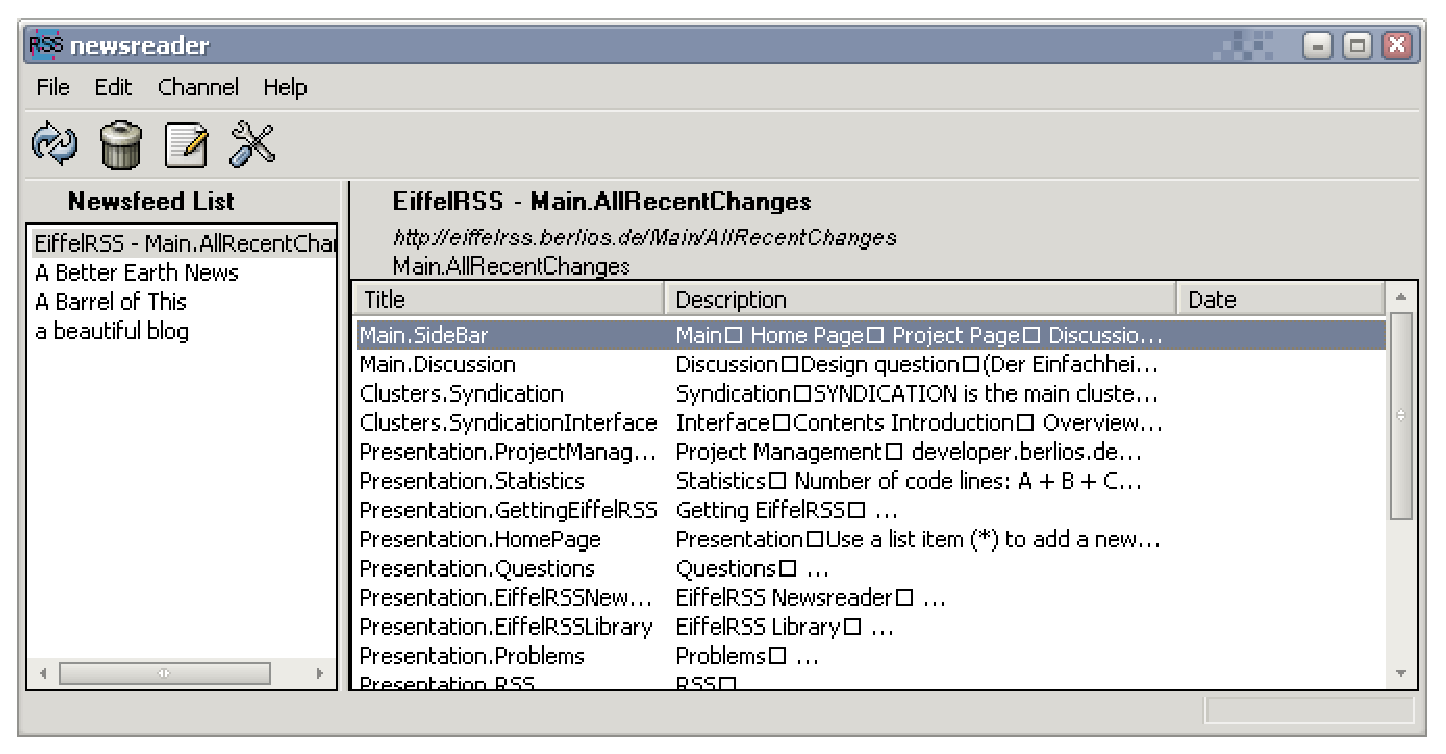
\includegraphics{figures/newsreader}}
      \end{center}

      \begin{center}
        \resizebox*{0.5\columnwidth}{!}{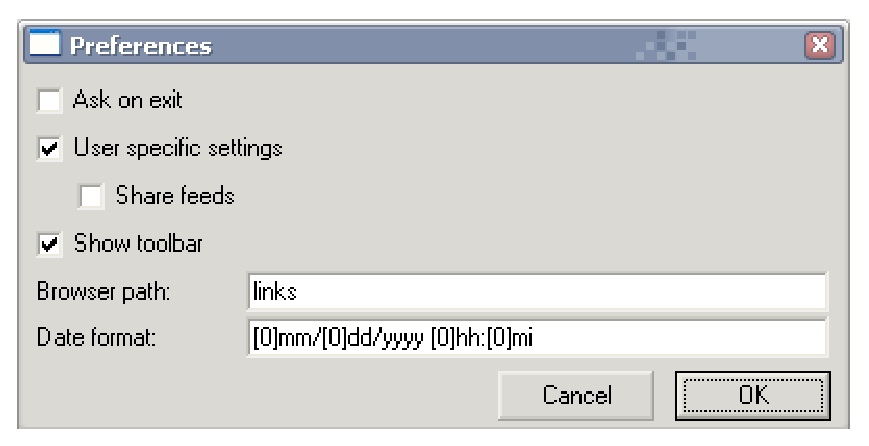
\includegraphics{figures/newsreader_preferences}}
      \end{center}
    }
  }

  \vspace{1cm}

  \fcolorbox{black}{backblue}
  {
    \parbox{1.0\columnwidth}
    {
      \section*{What is RSS?}

      \begin{itemize}
      \item RSS is an acronym for Really Simple Syndication, Rich Site
        Summary or RDF Site Summary
      \item It is a XML format for syndicating news, the content of
        news-like sites and pretty much anything that can be broken
        down into discrete items, e.g. the "recent changes" page of a
        Wiki, a changelog of SVN checkins, even the revision history
        of a book.
      \item Once information about each item is in RSS format, an
        RSS-aware program can check the feed for changes and react to
        the changes in an appropriate way.
      \item There are 9 different and incompatible versions of RSS
        (see
        http://diveintomark.org/archives/2004/02/04/incompatible-rss).
        \\
        EiffelRSS handles only RSS 2.0 at the moment, but can handle
        all of them through specialized reader and writer classes.
      \end{itemize}
    }
  }
  
  \vspace{1cm}

  \fcolorbox{black}{backblue}{
    \parbox{1.0\columnwidth}
    {
      \section*{Getting EiffelRSS}

      \begin{itemize}
      \item http://eiffelrss.berlios.de
      \item Subversion: svn checkout svn://svn.berlios.de/eiffelrss
      \end{itemize}
    }
  }
  
\end{multicols}

\vspace{0.5cm}


%-------------------------------------------------------------------------------
% Footer
%-------------------------------------------------------------------------------
\colorbox{qmuldarkblue} 
{
  \color{white}
  \parbox{1.0\textwidth}
  {
    \vspace{0.2cm}
  
    \begin{center}
      Produced using \LaTeX.
    \end{center}

    \vspace{0.2cm}
  }
}

\end{document}
